\section{Introdution}
\frametitle{Introdution}

  \begin{frame}{Introdution}
    \begin{itemize}
      \item \textbf{SCARA}
      \item Simulation using softwares(\textbf{MATLAB}, \textbf{Simulink})
      \item Kinematic Modeling(\textbf{Inverse Kinematics})
      \item Equations (\textbf{Actuador Modeling, Transmission Equations})
    \end{itemize}

  \end{frame}

  \begin{frame}{Introdution}
    \begin{columns}

      \begin{column}{0.6\textwidth}
        \begin{figure}
          \centering
          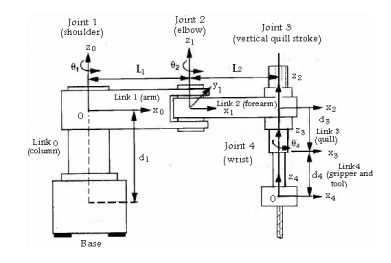
\includegraphics[width=1.05\textwidth]{fig/SCARA.png}
          \caption{Robot SCARA.}
        \end{figure}
      \end{column}

    \end{columns}

  \end{frame}